\documentclass[tikz,border=2pt]{standalone}


\begin{document}

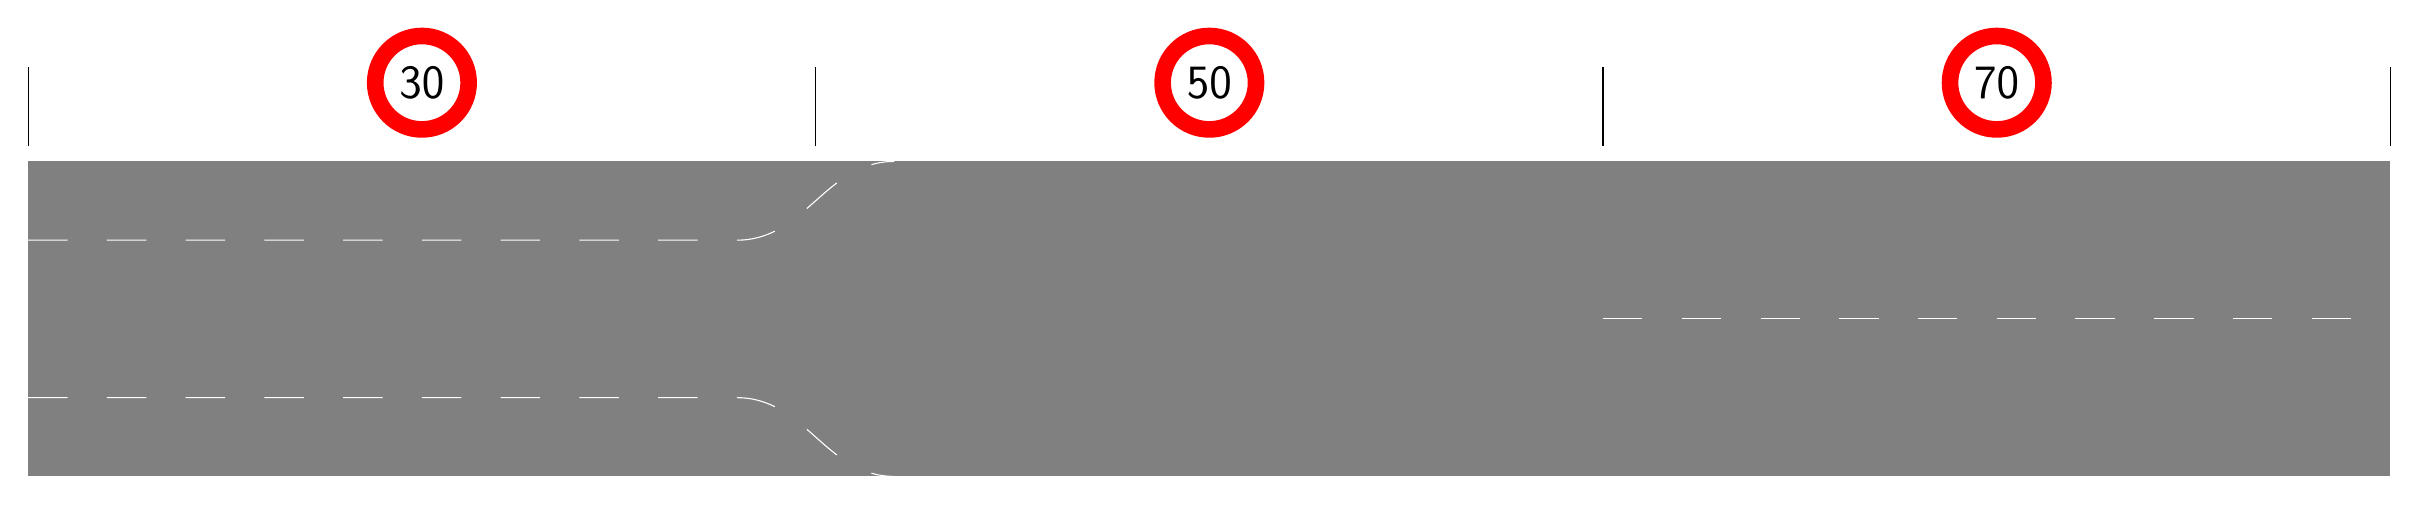
\begin{tikzpicture}[lijn/.style={dash=on .5cm off .5cm phase 0pt}
,bord/.style={circle,font=\LARGE\sffamily,line width=6pt,inner sep=5pt,preaction={draw=red}}
]
\fill[black!50] (0,0) rectangle (30,4);
\draw[white,lijn] (0,1) -- (9,1) to[in=180,out=0] (11,0);
\draw[white,lijn] (0,3) -- (9,3) to[in=180,out=0] (11,4);
\draw[white,lijn] (20,2) -- (30,2);
\draw (0,4.2) -- +(0,1) (10,4.2) -- +(0,1) (20,4.2) -- +(0,1) (30,4.2) -- +(0,1);
\node[bord] at ( 5,5) {30};
\node[bord] at (15,5) {50};
\node[bord] at (25,5) {70};
\end{tikzpicture}

\end{document}